\subsection{Analysing the new modules}
Our new sequential state space exploration algorithm  yields increasing speedups compared to PIPE 4 for small state spaces as can be seen in \cref{tbl:pipe5_vs_pipe4_sequential}. Interestingly the algorithm for the sequential exploration does not differ from that of PIPE 4, the speedup comes from advanced data structure usage, memoization and other optimisation techniques.

\begin{table}[tb]
\begin{center}
  \begin{tabular}{| c | c | c | c | c | }
  \hline
    Number of states & Number of transitions & PIPE 4 (s) & PIPE 5 (s) & Speedup \\
    \hline
    40 & 156 & 0.21 & 0.17 & 1.24\\
    \hline
    100 & 480 & 0.36 & 0.40 & 0.90\\
    \hline
    625 & 4000 & 25.12 & 1.35 & 18.61\\
    \hline
    1350 & 9450 & 83.67 & 1.75 & 47.81\\
    \hline
    4096 & 28672 & 728.02 & 3.82 & 190.58\\
    \hline
    11664 & 93312 & 2738.37 & 8.51 & 321.78\\
    \hline
  \end{tabular}
\caption{The time taken in seconds to generate the reachability graph in PIPE 4 compared with the new sequential algorithm in PIPE 5. For very small state spaces we can see that the times are comparable, but for moderate sized Petri nets PIPE 5 is more scalable.}
\label{tbl:pipe5_vs_pipe4_sequential}
\end{center}
\end{table}

% Next we compare our sequential algorithm to our MapReduce-style parallel algorithm running on 4 virtual cores. Since the underlying algorithm performed  is very similar we expect to see a linear speedup and indeed the results in \cref{fig:parallel_vs_sequential_algo} show approximately this. We allowed each worker thread to process 100, 200, 500 states before returning to have their results reduced and although there is little difference between them, the 100 states per thread run provides the best speedup against the sequential implementation. Using these results we went on to investigate the benefits for larger state spaces and observed that we see similar speedups in \cref{fig:pipe5_large_state_space}.

% \begin{figure}[tb]
\internal{}
\setfigname{}
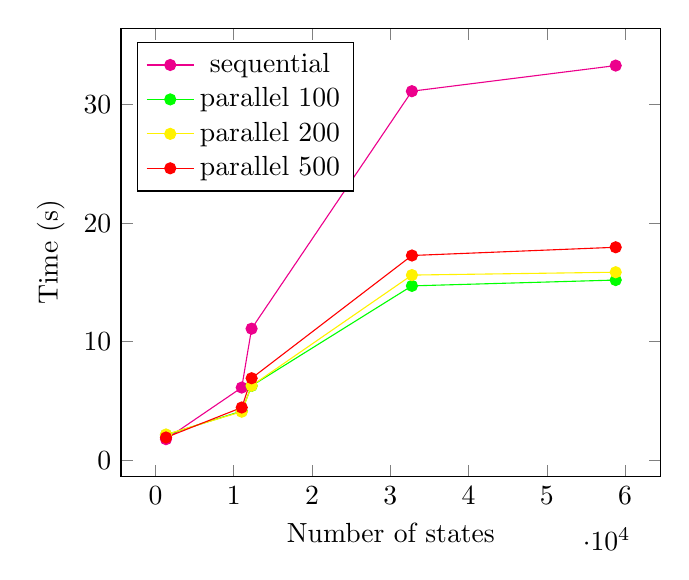
\begin{tikzpicture}
\definecolor{color0}{rgb}{0.75,0,0.75}

\begin{axis}[legend style={legend pos=north west},
ylabel={Time (s)},
xlabel={Number of states},
legend entries={{sequential},{parallel 100},{parallel 200},{parallel 500}}
% scaled ticks=false
]

% Sequential
\addplot [magenta, mark=*, mark size=2pt]
coordinates {
(1350,    1.783922000)
(11025,   6.135198000)
(12284,  11.098990000)
(32762,  31.121684000)
(58800,  33.280614000)
};

% 100
\addplot [green, mark=*, mark size=2pt]
coordinates {
(1350,   2.141683000)
(11025,  4.152756000)
(12288,  6.279725000)
(32768, 14.708286000)
(58800, 15.199168000)
};

% 200
\addplot [yellow, mark=*, mark size=2pt]
coordinates {
(1350,   2.177722000)
(11025,  4.099828000)
(12288,  6.293006000)
(32768, 15.619113000)
(58800, 15.858879000)
};

% 500
\addplot [red, mark=*, mark size=2pt]
coordinates {
(1350,   1.926380000)
(11025,  4.453230000)
(12288,  6.920561000)
(32768, 17.269375000)
(58800, 17.962744000)
};


\end{axis}
\end{tikzpicture}
\caption{A comparison between the run-times of PIPE 5's sequential state space exploration algorithm and the new MapReduce-style parallel algorithm running on 4 cores. We have allowed the parallel implementation to explore 500, 200, and 100 states before the reduction phase of each iteration. All parallel implementations yield at least a 2x speedup over the sequential algorithm although the 100 states per thread run performs slightly better than the others.}
\label{fig:parallel_vs_sequential_algo}
\end{figure}
% \begin{figure}[tb]
\internal{}
\setfigname{}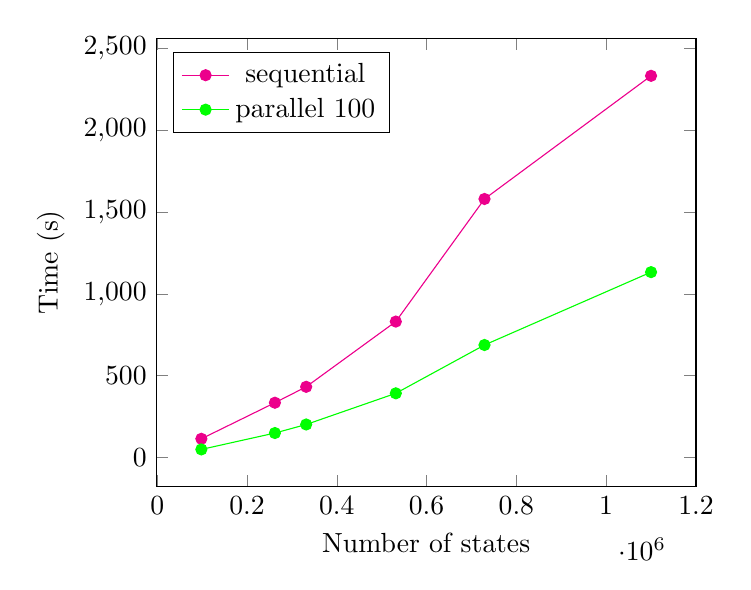
\begin{tikzpicture}
\definecolor{color0}{rgb}{0.75,0,0.75}

\begin{axis}[legend style={legend pos=north west},
ylabel={Time (s)},
xlabel={Number of states},
legend entries={{sequential},{parallel 100}}
% scaled ticks=false
]

% Sequential
\addplot [magenta, mark=*, mark size=2pt]
coordinates {
(98304,    113.690935000)
(262144,   334.272121000)
(331776,   431.582282000)
(531441,   830.441474000)
(729000,  1580.024665000)
(1099999, 2332.978991000)
};

% 100
\addplot [green, mark=*, mark size=2pt]
coordinates {
(98304,     48.798438000)
(262144,   148.977296000)
(331776,   201.183179000)
(531441,   391.800028000)
(729000,   687.234732000)
(1099999, 1132.697077000) % This is slightly over half an hr at 31 mins!
};

\end{axis}
\end{tikzpicture}
\caption{A comparison between the run-times of PIPE 5's sequential state space exploration algorithm and the new MapReduce-style parallel algorithm running on 4 cores for large Petri nets. This shows that the parallel implementation is consistently around twice as fast.}
\label{fig:pipe5_large_state_space}
\end{figure}

% Overall these results show a considerate speedup and allow for Petri nets with large state spaces to be analysed realistically on local machines.

To investigate the scalability of our parallel algorithm we analyse the new sequential and parallel algorithms against each other using a machine with a 3.40Ghz quad-core i7 processor. \cref{fig:scalability} shows that whilst the speedup from 2 to 4 virtual cores is promising at around 60\%, we do not get such good results from running the algorithm with 8 virtual cores. On profiling we found that the bottleneck in our algorithm is the creation of a states primary and secondary hash codes, taking 68\% of the algorithms run-time. Unfortunately since there is no implementation of a concurrent queue in Java that does not allow duplicates, we discovered that quite often it is possible to add a state twice to the exploration queue, meaning that its successors get generated twice too, causing their hash codes to be re-calculated.

\begin{figure}[ptb]
 \hspace*{\fill}%

\subcaptionbox{The raw times of the steady state exploration graph. The results gathered are for a sequential algorithm and for a parallel implementation with 100 states per thread running on 2, 4, and 8 virtual cores.} {
    \setfigname{}
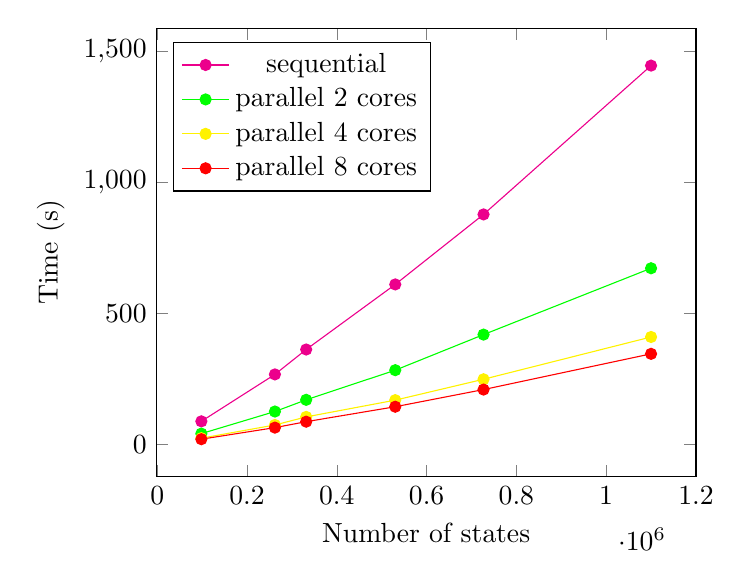
\begin{tikzpicture}
\definecolor{color0}{rgb}{0.75,0,0.75}

\begin{axis}[legend style={legend pos=north west},
ylabel={Time (s)},
xlabel={Number of states},
legend entries={{sequential},{parallel 2 cores},{parallel 4 cores},{parallel 8 cores}}
% scaled ticks=false
]

% Sequential
\addplot [magenta, mark=*, mark size=2pt]
coordinates {
(98279,     88.633369210) 
(262144,   267.658476596) 
(331776,   362.664597933) 
(530202,   610.926546563) 
(726836,   878.042343995) 
(1099999, 1445.821632163) 
};

% 2
\addplot [green, mark=*, mark size=2pt]
coordinates {
(98279,    41.786394435)
(262144,  126.064339906)
(331776,  170.664153825)
(530202,  283.808419361)
(726836,  419.506128369)
(1099999, 672.649284048)
};

% 4
\addplot [yellow, mark=*, mark size=2pt]
coordinates {
(98279,    24.373880968) 
(262144,   74.762257833) 
(331776,  105.559247500)
(530202,  169.459170682)
(726836,  249.133023117)
(1099999, 410.412285810)
};

% 8
\addplot [red, mark=*, mark size=2pt]
coordinates {
(98279,    20.521322935)  
(262144,   64.652309353)  
(331776,   87.323938113) 
(530202,  144.356493902) 
(726836,  209.819065630) 
(1099999, 346.097981548) 
};


\end{axis}
\end{tikzpicture}

}\hfill
\subcaptionbox{The relevant speedup gained over the sequential algorithm running our parallel algorithm with 100 states per thread and an increasing number of virtual cores. The graph shows that for each increase in the number of virtual cores we see a consistent speedup.} {
    \setfigname{}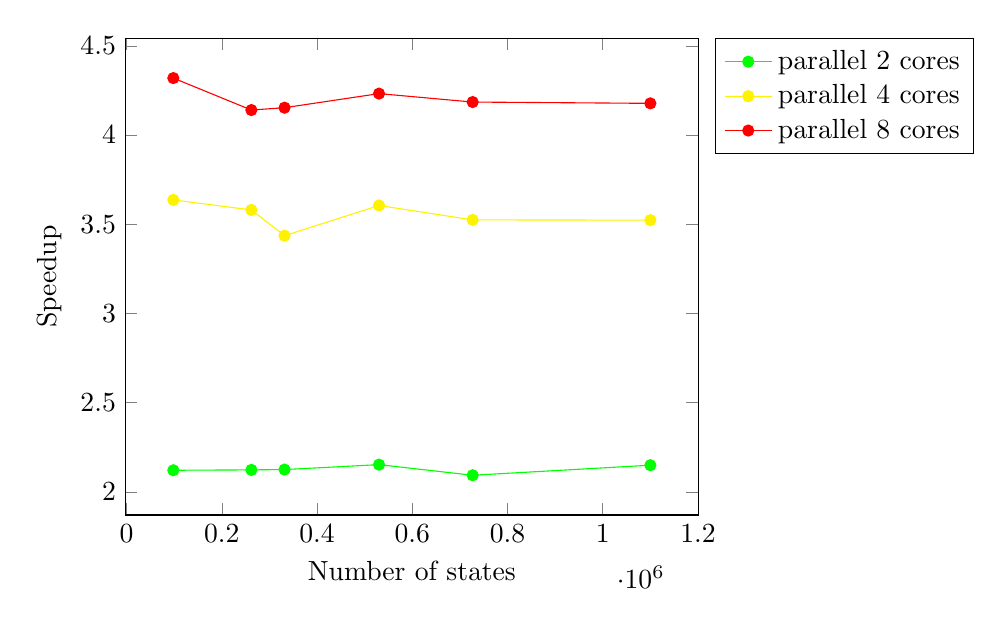
\begin{tikzpicture}
\definecolor{color0}{rgb}{0.75,0,0.75}

\begin{axis}[width=0.73\textwidth,
legend style={legend pos=outer north east},
ylabel={Speedup},
xlabel={Number of states},
legend entries={{parallel 2 cores},{parallel 4 cores},{parallel 8 cores}}
% scaled ticks=false
]

% 2
\addplot [green, mark=*, mark size=2pt]
coordinates {
(98279,   2.1211059343220406) % 99860326918 / 51611435904
(262144,  2.1231894506851012) % 304887660912 / 158793100442 
(331776,  2.1250191666193614) % 407267170985 / 208514610650
(530202,  2.152601913426362) % 709773626643 / 362338733157
(726836,  2.093038181369949) % 1023339231997 / 523542258224
(1099999, 2.149443501169068) % 1621045044327 / 845268409674
};

% 4
\addplot [yellow, mark=*, mark size=2pt]
coordinates {
(98279,   3.6364077319637786) % 99860326918 / 30575984607
(262144,  3.5801283208150485) % 304887660912 / 93863598681
(331776,  3.43564970878558) % 407267170985 / 127750195215
(530202,  3.605154823455611) % 709773626643 / 215606239138
(726836,  3.5243916402950974) % 1023339231997 / 318285464137
(1099999, 3.522851732641215) % 1621045044327 / 515475748470
};

% 8
\addplot [red, mark=*, mark size=2pt]
coordinates {
(98279,   4.319086517508672) % 99860326918 / 26825872545
(262144,  4.139967764099366) % 304887660912 / 82619391439
(331776,  4.153094853139814) % 407267170985 / 110556083237
(530202,  4.232068333397891) % 709773626643 / 189352805147
(726836,  4.184759575392262) % 1023339231997 / 282687963976
(1099999, 4.177492239903399) % 1621045044327 / 456685753436
};


\end{axis}
\end{tikzpicture}

}
\hspace*{\fill}%
\caption{A comparison between the run-times and relevant speedup of PIPE 5's sequential state space exploration and its parallel algorithm with 100 states per thread running on 2, 4 and 8 virtual cores on a 3.2GHz quad-core hyper-threaded 3rd generation i7 processor.}
\label{fig:scalability}
\end{figure}

Nevertheless in order to put into perspective the speedup gained by our new parallel algorithm using 100 states per thread and 8 virtual-cores we compared the run-times of a 4096 state Petri net with this algorithm and PIPE 4. Whilst PIPE 4 explores the state space in 9.37 minutes, our new algorithm can explore it in 2.65 seconds which amounts to an incredible 211x speedup. Moreover our new algorithm can solve a Petri net with \num{1099999} states in 5.77 minutes which is faster than the time taken to solve the 4096 state Petri net in PIPE 4!